\section{Methods}
\label{sec:methods}

This chapter provides an insight into the methodology used in this study.
First, the software tools and libraries that were employed for the study are presented.
Then the applied data preparation techniques are discussed in more detail.
Subsequently, each benchmark and experimental CNN method used in the study is thoroughly explained.
The chapter concludes with an examination of the performance metrics 
utilized for the evaluation of the research outcomes.

\subsection{Software Tools and Libraries}
\label{subsec:libs}

% Add versions of libraries!!!

The project was built on \textit{Python 3.10}.
A variety of widely adopted open-source libraries were used in the project.
\textit{NumPy} was utilized to perform efficient array operations and numerical calculations.
The \textit{NIBabel} library was used for reading and writing of medical image data stored in the
Neuroimaging Informatics Technology Initiative (NIfTI) file format.
\textit{PyTorch}, a widely adopted deep learning framework, was employed for building 
and training the neural networks.
The \textit{Torchvision} package provided the machine learning models and image transformation capabilities 
utilized in this project.
\textit{Pandas} was used for efficient structured data manipulation and analysis.
\textit{Matplotlib} and \textit{Seaborn} were employed for the creation of customized data visualizations.
The \textit{Scikit-Learn} library provided machine learning models and model evaluation tools utilized in this project, 
whereas \textit{Scipy} was used for data interpolation.

% seeds were set 
The seeds of the random number generators in each package were initialized to ensure reproducibility.

\subsection{Development Data Preparation}

\subsubsection{Data Preprocessing}
\label{subsubsec:img_preprocess_dev}

% Preprocessing of development dataset

% TODO -> wo "as described previously" -> näher beschreiben

Individual DAT-SPECT images were stereotactically normalized to the anatomical space of the Montreal Neurological Institute (MNI) 
using the Normalize tool of the Statistical Parametric Mapping software package (version SPM12) and a set of custom DAT-SPECT templates 
representative of normal and different levels of Parkinson-typical reduction of striatal uptake as target~\citep{Apostolova2023-ec}.
The voxel size of the stereotactically normalized images was 2x2x2 mm$^{3}$. 
Intensity normalization was achieved by voxelwise scaling to the individual $75^{\text{th}}$ percentile of the voxel intensity in a reference region 
comprising the whole brain without striata, thalamus, medial temporal lobe, brainstem, cerebellum, and ventricles~\citep{Kupitz2014-ll}.
The resulting images are distribution volume (DVR) images. 
A 2-dimensional transversal DVR slab of 12mm thickness and 91x109 pixels with 2 mm edge length was obtained 
by averaging 6 transversal slices through the striatum~\citep{Buchert2006-pt}.

\subsubsection{Data Augmentation}
\label{subsec:augment}

Data augmentation was applied to the development dataset to increase the heterogeneity of the data.
To enhance robustness across various attenuation correction and scatter correction methods, 
each image was generated in a version with and without attenuation and scatter corrections applied~\citep{Schiebler2023}.
Also, 3D-smoothing of the 3-dimensional SPECT images in MNI space 
was performed before computing the 2-dimensional slabs as an augmentation technique.
A 3-dimensional isotropic Gaussian kernel with various Full Width at Half Maximum (FWHM) 
values (FWHM = 10, 12, 14, 16, 18mm) was used for the smoothing.
Thereby an augmented dataset of 20,880 images in total was constructed based on 1,740 cases.
Two representative cases augmented using the described techniques are depicted in Figure~\ref{fig:dev_dataset}.

\begin{figure}[t]
    \centering
    \includegraphics[width=0.95\textwidth]{content/figures/dev_dataset.png}
    \caption{DVR slabs for two sample cases from the development dataset, 
    a healthy control case (above) and a PD case with reduced availability of DAT in the striatum (below).
    The two cases are presented in 12 different versions.
    In each version, attenuation and scatter corrections are either applied (`withASC') or not applied (`woASC').
    Also, for each version, isotropic 3-dimensional Gaussian kernel smoothing with different FWHM values (10, 12, 14, 16, 18mm) was 
    either performed or not performed (`original').} 
    \label{fig:dev_dataset}
\end{figure}

\subsubsection{Dataset Splitting}
\label{subsec:split}

% How was dev dataset split
Ten distinct random splits were created from the augmented development dataset, 
resulting in ten different combinations of training, validation, and test sets for the conducted experiments.
In each random split, the data distribution was as follows: 
60\% for the training set, 20\% for the validation set, and 20\% for the test set.
While splitting the data it was ensured that all augmented images associated with a given patient were put 
into the same subset.
Thereby, randomization into training, validation and test set was performed 
on the level of patients rather than on the level of single images.
Thereby inter-subset leakage of images from the same patient was avoided.

\subsection{Univariate benchmark: Specific Binding Ratio}
\label{subsec:sbr}

The unilateral [$^{123}$I]FP-CIT specific binding ratio (SBR) was used as a benchmark classification method.
Here, the SBR in left and right putamen was obtained by hottest voxels (HV) analysis of the stereotactically normalized 
DVR image using large unilateral putamen masks predefined in MNI space~\citep{Wenzel2019}.
The unilateral hottest voxel SBR was calculated as

\begin{equation}\label{eq:sbr}
  \text{HV-SBR}_{\text{unilateral}} = \left( \frac{1}{K_{\text{10ml}}} \sum_{k} \hat{I}_{k, ROI} \right) - 1 \;,
\end{equation}

where $\hat{I}_{k, ROI}$ represent the \textit{normalized} voxel intensities of the $K_{\text{10ml}}$
hottest voxels (i.e., voxels with the highest intensity) comprising a total volume of 10 ml 
within the unilateral putamen ROI in the DVR image.
The voxel intensities of the hottest voxels are normalized to the $75^{\text{th}}$ percentile of the voxel intensities 
in the reference region associated with non-specific binding~\citep{Wenzel2019}.
The minimum of the HV-SBR values from the left and right hemispheres of the brain was used for the analysis.
An in-depth elaboration on SBR analysis can be found in~\cite{Wenzel2019}.

The SBR-based classifier was obtained for each of the random splits (n = 10) as follows.
First, the optimal cutoff on the SBR was determined in the validation set
using ROC analysis and the Youden criterion~\citep{Youden1950}.
The determined optimal cutoff was then used as the decision boundary between normal control cases and Parkinson's disease 
and evaluated on the test set of the development dataset.
Also, the determined cutoff was evaluated on the PPMI and MPH test datasets described in Section~\ref{subsec:external_dataset}.
As a result, 10 optimal cutoffs on the SBR were determined and evaluated.

\subsection{Multivariate benchmark: PCA-enhanced Random Forest}
\label{subsec:pca_rfc}

As a further benchmark, a random forest classifier was trained on PCA-transformed features of the training set 
of the development dataset.

To be comparable with CNN-based approaches, first, a 91x91 pixel square-shaped region of interest 
was defined within the 91x109 pixel DVR slab, and each development data image (of each subset) was cropped to this region.
The square-shaped region was determined by cropping an equal number of pixels from the top and bottom 
of the DVR slab along its second dimension (anterior-posterior direction).
The used region of interest is marked in Figure~\ref{fig:dev_dataset}.

Then a PCA model with 10 principle components was initialized and fit to the training set to obtain 
the principle components of the training set.
The determined principle components were used to transform the training set into a lower-dimensional space,
where each image was represented by a 10-vector characterizing the expression of each principal component.
An example of the principle components of the training set for one of the random splits is depicted in Figure~\ref{fig:pca_components}.

The training data transformed by the principle components was then used to train a random forest classifier with 100 decision trees.
As hyperparameters, the Gini impurity was used to assess split quality, 
with a minimum of 2 samples required to split an internal node and 1 sample needed at a leaf node.
The trained random forest classifier was evaluated on the test split of the development dataset for each of the 10 random splits.
In addition, the trained model was tested on the PPMI and MPH datasets described in Section~\ref{subsec:external_dataset}.

\begin{figure}[ht]
  \centering
  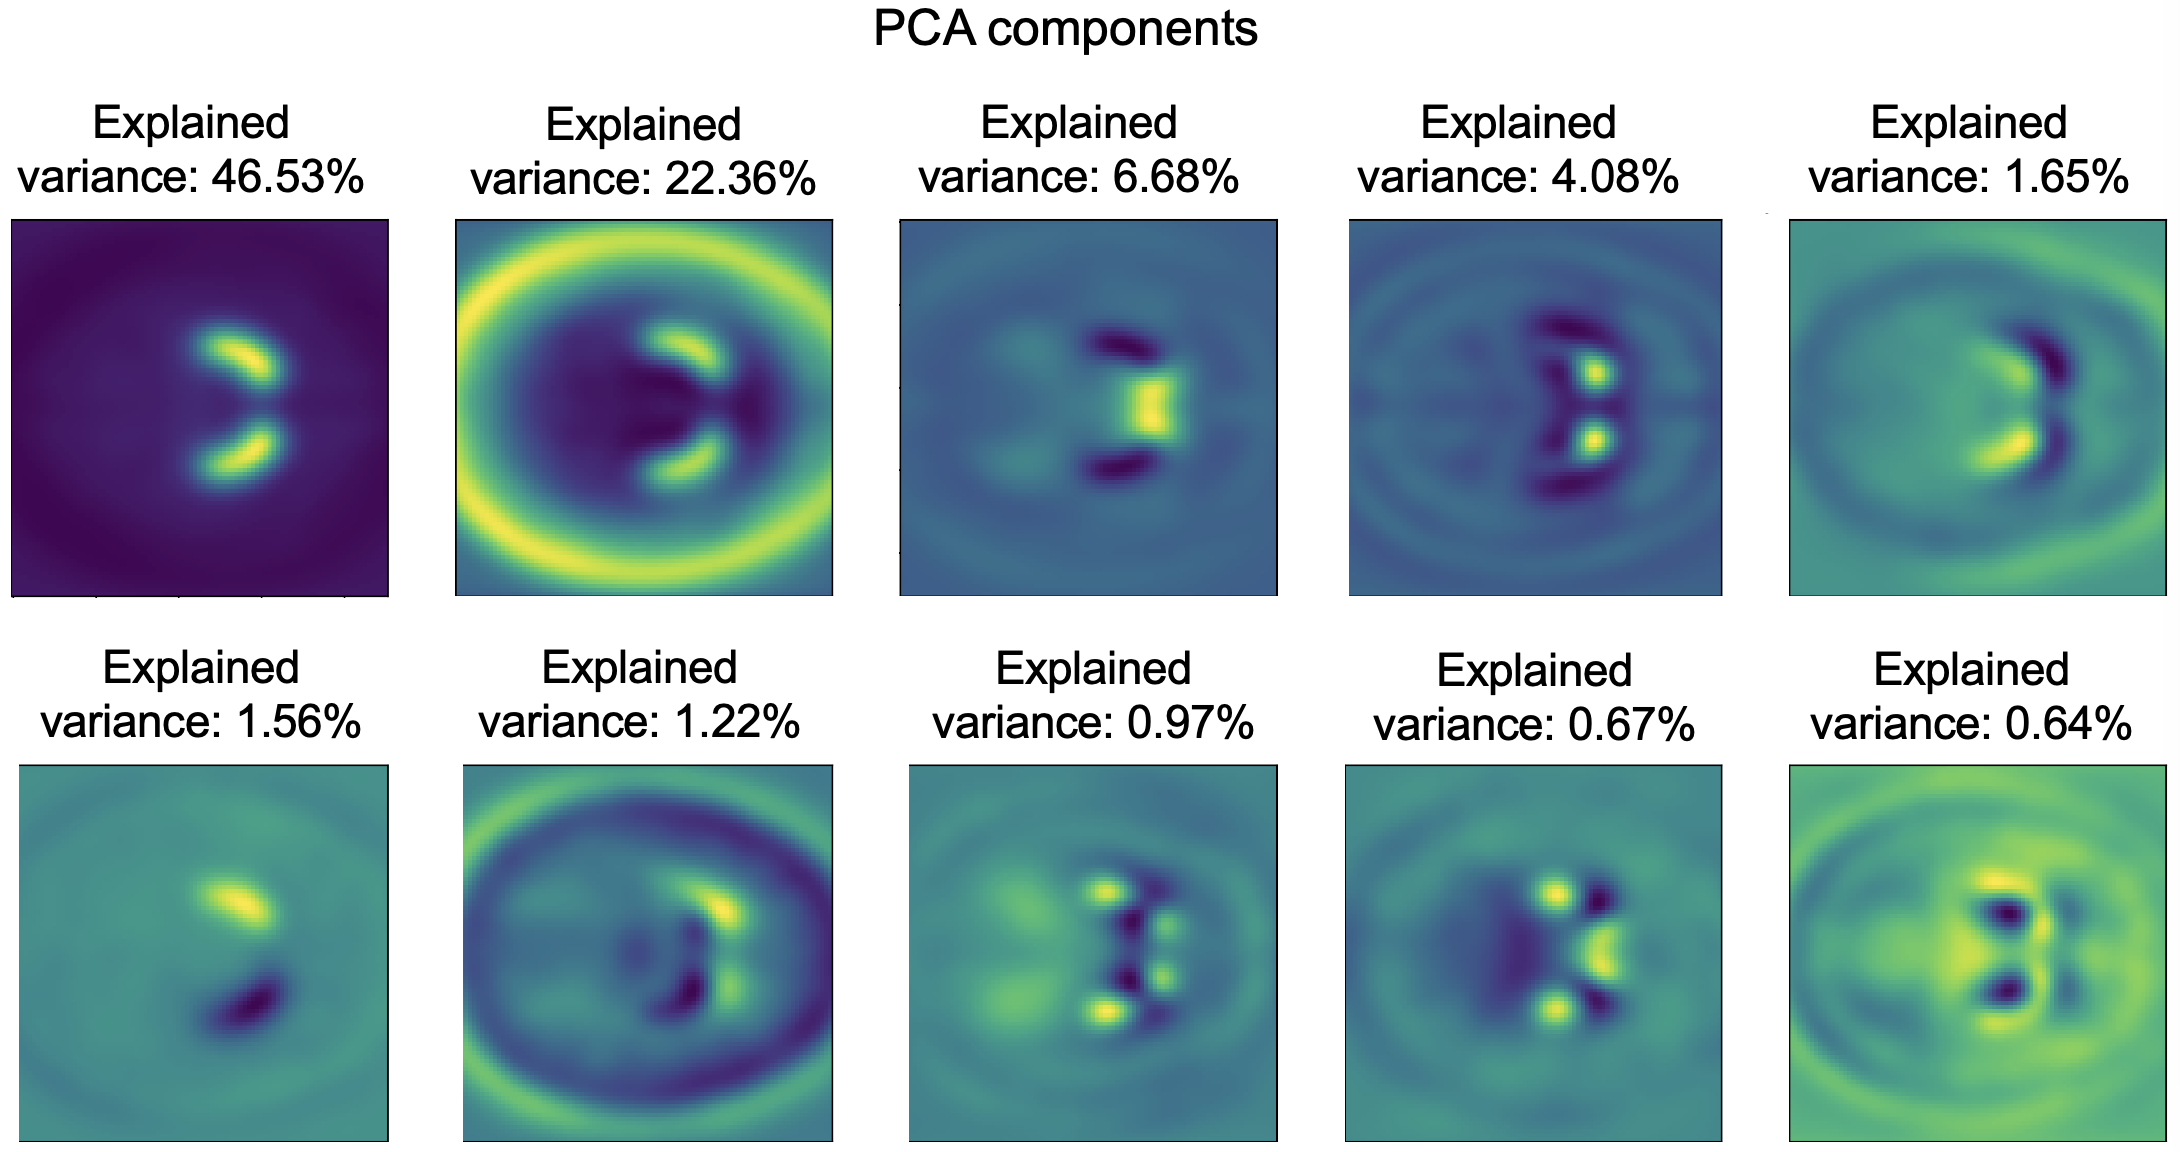
\includegraphics[width=1.0\textwidth]{content/figures/pca_components_splittrain_enhanced.png}
  \caption{Principle components of the training set (development dataset) for the first random split.
  The principle components are arranged in descending order based on the amount of variance they explain.} 
  \label{fig:pca_components}
\end{figure} 

\subsection{CNN-based classification}
\label{subsec:cnn_based_classification}

% Model architecture
The models of CNN-based classifiers were based on a Residual Network (ResNet) architecture.
More precisely, the \textit{ResNet-18}~\citep{resnet2015} model architecture consisting of 18 layers was used as basis.
The non-pretrained weights of the ResNet-18 were used as initial weights.
The ResNet-18 architecture expects input tensors of size (3, 224, 224), 
denoting images with 3 channels and spatial dimensions of 224 by 224 pixels.
Since the development data has one color channel, the architecture was modified to expect one input channel at its 
first convolutional layer.
Also the dimensions of the last fully-connected layer of the architecture were modified to produce one output node 
in the output layer.
The modified ResNet-18 model is depicted in Figure~\ref{fig:resnet}.
To produce a probabilistic model output within the range of $0$ to $1$, 
the sigmoid function was applied to the output layer of the model.

% Required preprocessing for CNN: ROI cropping and interpolation to (224, 224)
Further development data preprocessing was performed to comply with the spatial input 
dimensions required by the model architecture.
First, a 91x91 pixel square-shaped region of interest was defined within the 91x109 pixel DVR slab, 
and each development data image (of each subset) was cropped to this region.
The cropping to a square shape was performed to preserve the aspect ratio while doing the subsequent upscaling.
The square-shaped region was determined by cropping an equal number of pixels from the top and bottom 
of the DVR slab along its height dimension.
Then the square-shaped images were resized to the target image size of 224x224 pixels using bicubic interpolation.

The CNN-based methods were trained for $20$ epochs using a batch size of $64$.
For the MVT and RLT approaches (described in Section~\ref{subsubsec:cnn_based_classification_mvt_rlt}) 
the Binary Cross Entropy (BCE) loss was employed for optimization, 
whereas for the Regression approach (described in Section~\ref{subsubsec:cnn_based_classification_regression}) 
the Mean Squared Error (MSE) loss function was used.
The Adam optimization algorithm was utilized with an initial learning rate of $0.0001$.
No hyperparameter optimization was conducted for the CNN-based methods.
During the training of the model, the weights of the best epoch were saved for subsequent evaluations.
Each CNN model was trained and evaluated separately for each of the $10$ random splits of the development dataset.
Additionally, the trained models were evaluated on the PPMI and MPH test datasets described in Section~\ref{subsec:external_dataset}.
No attempt was made to adapt the CNN models trained in the development dataset for these independent test datasets.

\begin{figure}[t]
  \centering
  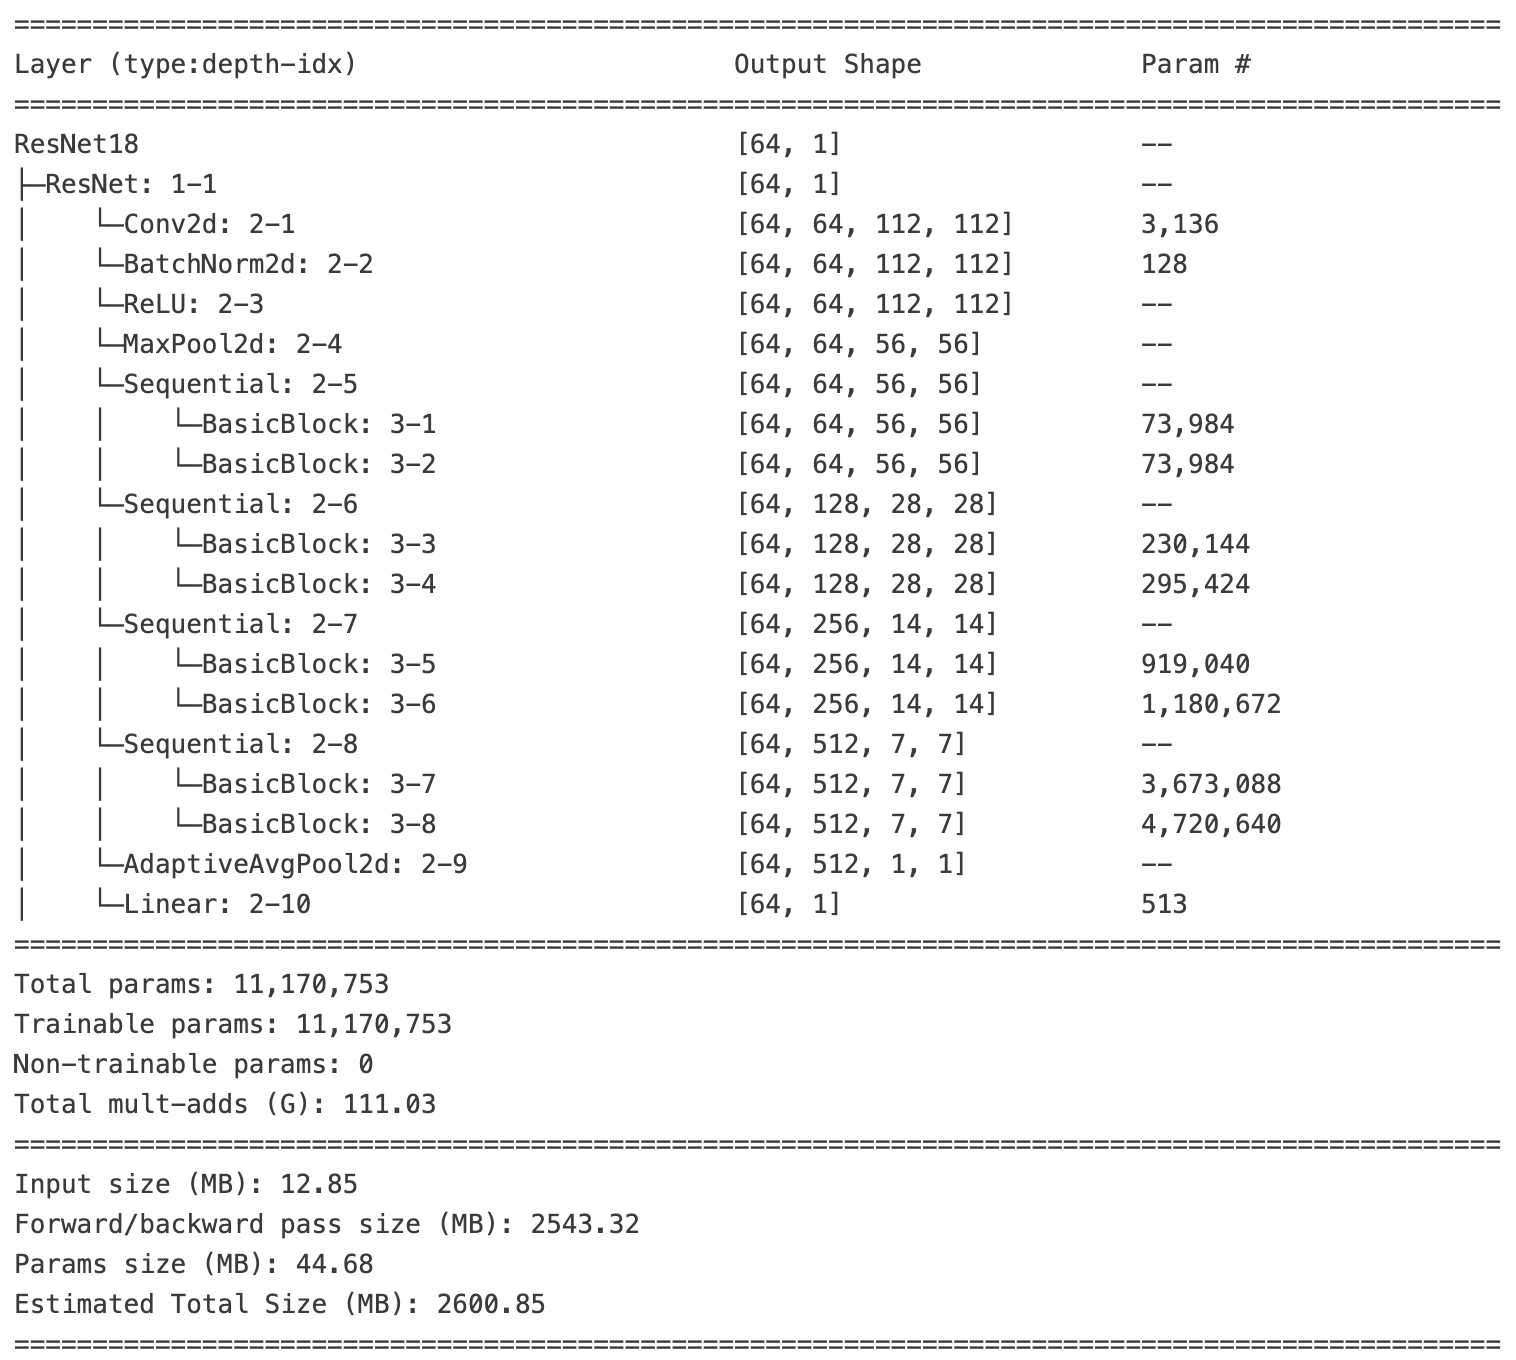
\includegraphics[width=1.0\textwidth]{content/figures/cnn_architecture.png}
  \caption{Architecture of the CNN-based classification models.} 
  \label{fig:resnet}
\end{figure} 

\subsubsection{MVT-based and RLT-based methods}
\label{subsubsec:cnn_based_classification_mvt_rlt}

When training a CNN using the BCE loss function, 
one has to provide the ground truth label of each instance to the optimization algorithm.
Given that each instance in the development data is labeled by three independent readers, 
a selection strategy must be determined.
The following two label selection strategies are used for training the CNNs: 
Majority Vote training (MVT) and Random Label training (RLT).
The labels chosen using one of the two strategies are then used, together with the model predictions, 
to compute the BCE loss.

% MVT
Majority vote training involved selecting the label that received the majority of votes from the readers as the 
ground truth label.
Since there are three available labels, 
a majority is reached when two out of the three readers agree on a particular label (e.g., the normal case (NC)).
During the model training phase, the majority vote strategy was employed to select the labels for both the training 
and validation data instances.

% RLT
In contrast to MVT, random label training involved choosing a random label from the three available options
as the ground truth label.
The seed of the random number generator (responsible for the random selection) is set only once at the start of the
algorithm and is not reset between the model training epochs.
Thereby a different label could be chosen as the ground truth label for each distinct training epoch.
Here the random label selection strategy is applied both to the training and validation data.
% majority on validation better?

\subsubsection{Regression-based method}
\label{subsubsec:cnn_based_classification_regression}

The regression-based approach aimed to incorporate the uncertainty regarding the ground truth label 
into the training algorithm.
The ground-truth label was derived from the combination of the three available labels, 
resulting in a floating-point number.
Each of the following states of certainty about the label was mapped to a distinct 
floating-point valued ground-truth label: 
\emph{all readers agree on `normal' } (ground-truth label: 0.0), 
\emph{majority of readers (two out of three) agree on `normal'} (ground-truth label: 1.0/3.0), 
\emph{majority of readers (two out of three) agree on `reduced'} (ground-truth label: 2.0/3.0) 
and \emph{all readers agree on `reduced'} (ground-truth label: 1.0).
This mapping of available labels to the ground-truth label was used for both the training 
and validation data during the model training phase.

During model training, the loss was computed using the Mean Square Error loss function 
which aims to minimize the mean of the squared differences between the model predictions and the ground-truth labels.
%Thereby the optimization algorithm aimed to separate cases where no consensus was reached from those where consensus was achieved.

\subsection{Evaluation Metrics and Procedure}
\label{subsec:eval_metrics_proced}

In the following the performance metrics used for the evaluation of the different classification methods 
are explained in more detail.

First the $\text{mean} \pm \text{SD}$ (standard deviation) of the following measures were calculated across
the different random splits for each classification approach and subset (training, validation and testing) given a cutoff: 
AUC-ROC, balanced accuracy, (overall) accuracy, sensitivity, specificity, PPV and NPV.
The natural cutoff of 0.5 was used for each classification approach except the SBR method.
For the SBR method the optimal cutoff was determined using the Youden criterion~\citep{Youden1950} and was used for
calculating the measures.
In the test set of the development dataset (for each random split),
the majority vote was used as ground truth in all cases.

% Determination of inconclusive intervals given set of percentages of inconclusive cases
Second, for each element within a set of considered percentages of inconclusive cases in the validation set (PIncVal)
the corresponding inconclusive interval was determined.
Inconclusive cases were defined as cases predicted within an inconclusive interval 
(bounded by lower and upper bound), while conclusive cases were those predicted outside this interval.
The determination of the inconclusive interval was exclusively performed using the validation set 
for each random split and classification approach independently.
The set of PIncVal values considered ranged from 0.2\% to 20.0\%, increasing in increments of 0.2\%.
For each target PIncVal value the lower and upper bounds of the inconclusive interval 
were independently determined in such a way that there was the same number of inconclusive cases ($\pm 1$ case) 
below and above the pre-defined cutoff.
For the CNN-based classification methods and the multivariate benchmark the natural cutoff of 0.5 was used,
whereas for the SBR-based univariate benchmark the optimal cutoff on the SBR was used.

% lower_bound(PIncVal) , upper_bound(PIncVal)
To assess the stability of the determined inconclusive interval over the proportion of inconclusive cases,
the determined upper and lower bounds ($\text{mean} \pm \text{SD}$ across the 10 random splits) 
of the inconclusive interval were plotted against the corresponding PIncVal (\%).
The rate at which the lower (upper) bound decreases (increases) over the PIncVal 
reflects the density of inconclusive cases within a certain region of PIncVal.
Specifically, higher function gradients indicate lower concentration of predictions, 
and vice versa.
Also, a higher standard deviation indicates that the stable inconclusive interval determination 
is less robust within a certain region of PIncVal.

% AUC of bal_acc vs. %inconclusive_cases; determination of inconclusive ranges for each %inconclusive_cases

As the main performance metric (regarding the primary hypothesis of the project) 
we propose the area under the curve of mean balanced accuracy (AUC-bACC, \%) on conclusive test cases 
as a function of the mean percentage of inconclusive test cases (mean PIncObs, \%).
More precisely the relative AUC-bACC (\%) normalized to the maximum achievable area was used for the comparison.
To obtain the relative AUC-bACC, 
first, the mean balanced accuracy function was interpolated using cubic spline interpolation.
Then the area under the mean balanced accuracy curve was computed using the trapezoidal rule 
and then normalized to the maximum achievable area (100\% balanced accuracy * (20\% - 0.2\%) inconclusive cases).
The evaluation of each classification method with respect to this metric was conducted on the test set of the 
development dataset as well as on the independent datasets PPMI and MPH.

% PIncObs(PIncVal) 
As a further metric, the $\text{mean} \pm \text{SD}$ percentage of observed inconclusive cases in the test set (PIncObs, \%) 
was plotted against the PIncVal (\%).
A mean of PIncObs(PIncVal) near the identity line is an indicator for a similar prediction distribution 
for validation set and test set on average.
In case the mean of PIncObs(PIncVal) consistently lies over (under) the identity line 
the supposed prediction certainty on the test set, on average, is lower (higher) than on the validation set.
Also a lower standard deviation of PIncObs over PIncVal indicates 
that PIncObs is less sensitive to the randomness of the inconclusive intervals across random splits.
In particular, a lower standard deviation of PIncObs allows for a more reliable calculation of the main performance metric.
